\documentclass[11pt]{report}
\usepackage[utf8]{inputenc}
\usepackage[T1]{fontenc}
 \usepackage{listings}

\usepackage{fancyhdr}
\usepackage{graphicx}
\usepackage{color}
\pagestyle{fancy}


 \lhead{Geoffrey PERRIN - Océane DUBOIS}
 \rhead{}
 \rfoot{}



\definecolor{codegreen}{rgb}{0,0.6,0}
\definecolor{codegray}{rgb}{0.5,0.5,0.5}
\definecolor{codepurple}{rgb}{0.58,0,0.82}
\definecolor{backcolour}{rgb}{0.95,0.95,0.92}

\lstdefinestyle{mystyle}{
    backgroundcolor=\color{backcolour},
    commentstyle=\color{codegreen},
    keywordstyle=\color{magenta},
    numberstyle=\tiny\color{codegray},
    stringstyle=\color{codepurple},
    basicstyle=\footnotesize,
    breakatwhitespace=false,
    commentstyle=\color{codegreen},   
    breaklines=true,
    captionpos=b,
    keepspaces=true,
    keywordsprefix= ; ,
    numbers=left,
    numbersep=5pt,
    showspaces=false,
    showstringspaces=false,
    showtabs=false,
    tabsize=2,
     morekeywords={mov, push, xor, extern, div, mov, inc, cmp, jne, call, pop, ret,endp, proc, end, dec, add, jb, dd, db, jge  not, lea, main, public, movzx,ABCD,ADD,%
ADDA,ADDI,ADDQ,ADDX,AND,ANDI,ASL,ASR,BCC,BLS,BCS,BLT,BEQ,BMI,BF,BNE,BGE,BPL,%
BGT,BT,BHI,BVC,BLE,BVS,BCHG,BCLR,BRA,BSET,BSR,BTST,CHK,CLR,CMP,CMPA,CMPI,CMPM,%
DBCC,DBLS,DBCS,DBLT,DBEQ,DBMI,DBF,DBNE,DBGE,DBPL,DBGT,DBT,DBHI,DBVC,DBLE,DBVS,DIVS,%
DIVU,EOR,EORI,EXG,EXT,ILLEGAL,JMP,JSR,LEA,LINK,LSL,LSR,MOVE,MOVEA,MOVEM,MOVEP,MOVEQ,%
MULS,MULU,NBCD,NEG,NEGX,NOP,NOT,OR,ORI,PEA,RESET,ROL,ROR,ROXL,ROXR,RTE,RTR,RTS,SBCD,%
SCC,SLS,SCS,SLT,SEQ,SMI,SF,SNE,SGE,SPL,SGT,ST,SHI,SVC,SLE,SVS,STOP,SUB,SUBA,SUBI,SUBQ,%
SUBX,SWAP,TAS,TRAP,TRAPV,TST,UNLK},
    extendedchars=true,
     sensitive=false,
   morecomment=[l]*,
   morecomment=[l]; ,
    literate= {á}{{\'a}}1 {é}{{\'e}}1 {í}{{\'i}}1 {ó}{{\'o}}1 {ú}{{\'u}}1 {Á}{{\'A}}1 {É}{{\'E}}1 {Í}{{\'I}}1 {Ó}{{\'O}}1 {Ú}{{\'U}}1 {à}{{\`a}}1 {è}{{\`e}}1 {ì}{{\`i}}1 {ò}{{\`o}}1 {ù}{{\`u}}1 {À}{{\`A}}1 {È}{{\'E}}1 {Ì}{{\`I}}1 {Ò}{{\`O}}1 {Ù}{{\`U}}1 {ä}{{\"a}}1 {ë}{{\"e}}1 {ï}{{\"i}}1 {ö}{{\"o}}1 {ü}{{\"u}}1 {Ä}{{\"A}}1 {Ë}{{\"E}}1 {Ï}{{\"I}}1 {Ö}{{\"O}}1 {Ü}{{\"U}}1 {â}{{\^a}}1 {ê}{{\^e}}1 {î}{{\^i}}1 {ô}{{\^o}}1 {û}{{\^u}}1 {Â}{{\^A}}1 {Ê}{{\^E}}1 {Î}{{\^I}}1 {Ô}{{\^O}}1 {Û}{{\^U}}1,
  }

\lstset{style=mystyle}

%Gummi|065|=)
\title{\textbf{TP03 - Prise en main de l'environement de développement assembleur et premiers programmes }
\author{Geoffrey PERRIN \\ Océane DUBOIS\\}
\date{}}

\begin{document}

\maketitle

\newpage

\section{Exercices : affichage de chaîne de caractère}

\subsection{Programme "Hello World"}

Dans le fichier "hello1.asm", la variable msg est définie comme un suite de bytes contenant "bonjour tout le monde".
La variable longueure est définie comme un data double word (il occupe ainsi tout un registre) contenant la valeur 21 soit le nombre de caractères (occupant chacun un byte) de la chaîne de caractère msg.

Le programme fonctionne donc ainsi :
\begin{itemize}
\item La fonction main (seule fonction du programme), commence par réaliser une sauvegarde pour le code 'C' grâce à push ebx (le contenu de ebx est mis sur le sommet de la pile) 

\item puis le registre ebx est mis à 0
\item puis on définie la ligne de programme qui suit avec l'étiquette "suivant". Cet ligne permet de mettre dans eax le contenu de l'adresse pointée par la somme de ebx et l'adresse de message. Le reste du registre sera completé par des zéros. Ebx va ici nous servir de controleur pour le nombre d'itération effectuées.
\item puis on met sur la pile le caratère à afficher et on appel la fonction c "putchar" qui elle-meme appelle fputchar qui permet d'afficher le caractère qui à été mis sur la pile.
\item puis on ajoute 4 au pointeur de pile pour le déplacer sur un emplacement non encore utilisé par le programme
\item on incrémente ensuite notre itérateur ebx
\item on effecture la comparaison entre ebx et la valeur contenue dans la variable longueure, les drapeaux sont mis à jour
\item si ebx et la valeur de longeur ne sont pas égaux cela signifie qu'on est pas arrivé à la fin de la chaine de caractère, on retourne donc à la ligne du programme ayant comme étiquette suivante et on réalise cette boucle jusqu'a ce que la valeur de longueure soit égale à la valeur de ebx.
\item si ebx et le contenu de longueur sont égaux on peut appeler la fonction c getchar qui attent l'appui sur "Entrée"
\item on met le sommet de la pile dans ebx
\item on signal au programme qu'il peut retourner au code de démarrage 'C' puis on fini le programme avec l'instruction "main endp"

\end{itemize}

Le fonctionnement de cet algorithme pourrait ressembler au fonctionnement d'un programme contenant l'instruction "while(ebx != longueur) en C. Et comme déjà dit précédement ebx nous sert d'itérateur (et donc la condition d'arrêt dépent de lui).


\begin{figure}[ht]
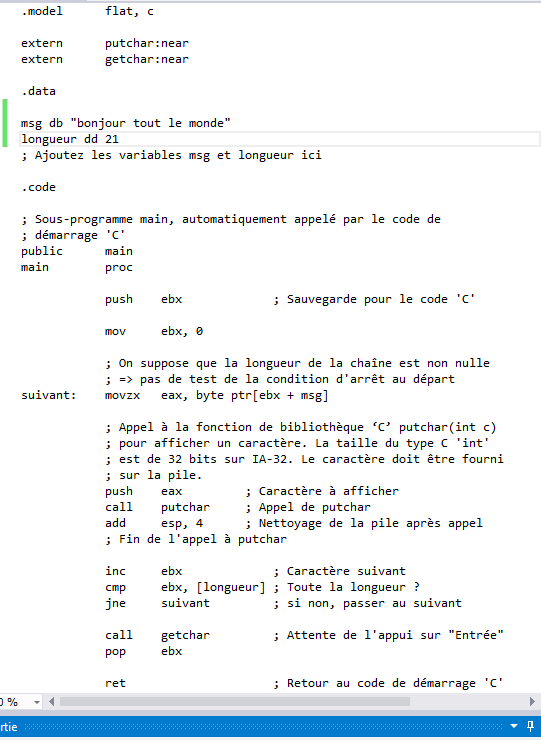
\includegraphics[width=8cm]{Capture5.PNG}
\caption{Programme "hello1"}
\end{figure}


\subsection{Chaîne de taille variable}

On modifie maintenant le premier code en "hello2" dans lequel la variable longueure n'est plus utilisée, à la place on définie la variable msg comme la chaine de caractère "bonjour tout le monde", terminée par un 0.

Nous avons donc modifié le programme pour qu'il affiche toujours correctement le contenu de msg. Pour cela on garde ebx qui nous sert toujours de variable permettant de parcourir chaque caractère du message à afficher. Mais la comparaison se fait entre eax et 0 en effet si eax est égal à 0 cela signifie qu'on est arrivé à la fin du message (cela est valable car la chaîne message ne contient pas de caractère 0).

L'algorithme implémenté correspond donc à un while(msg[ebx] != 0)



\begin{figure}[ht]
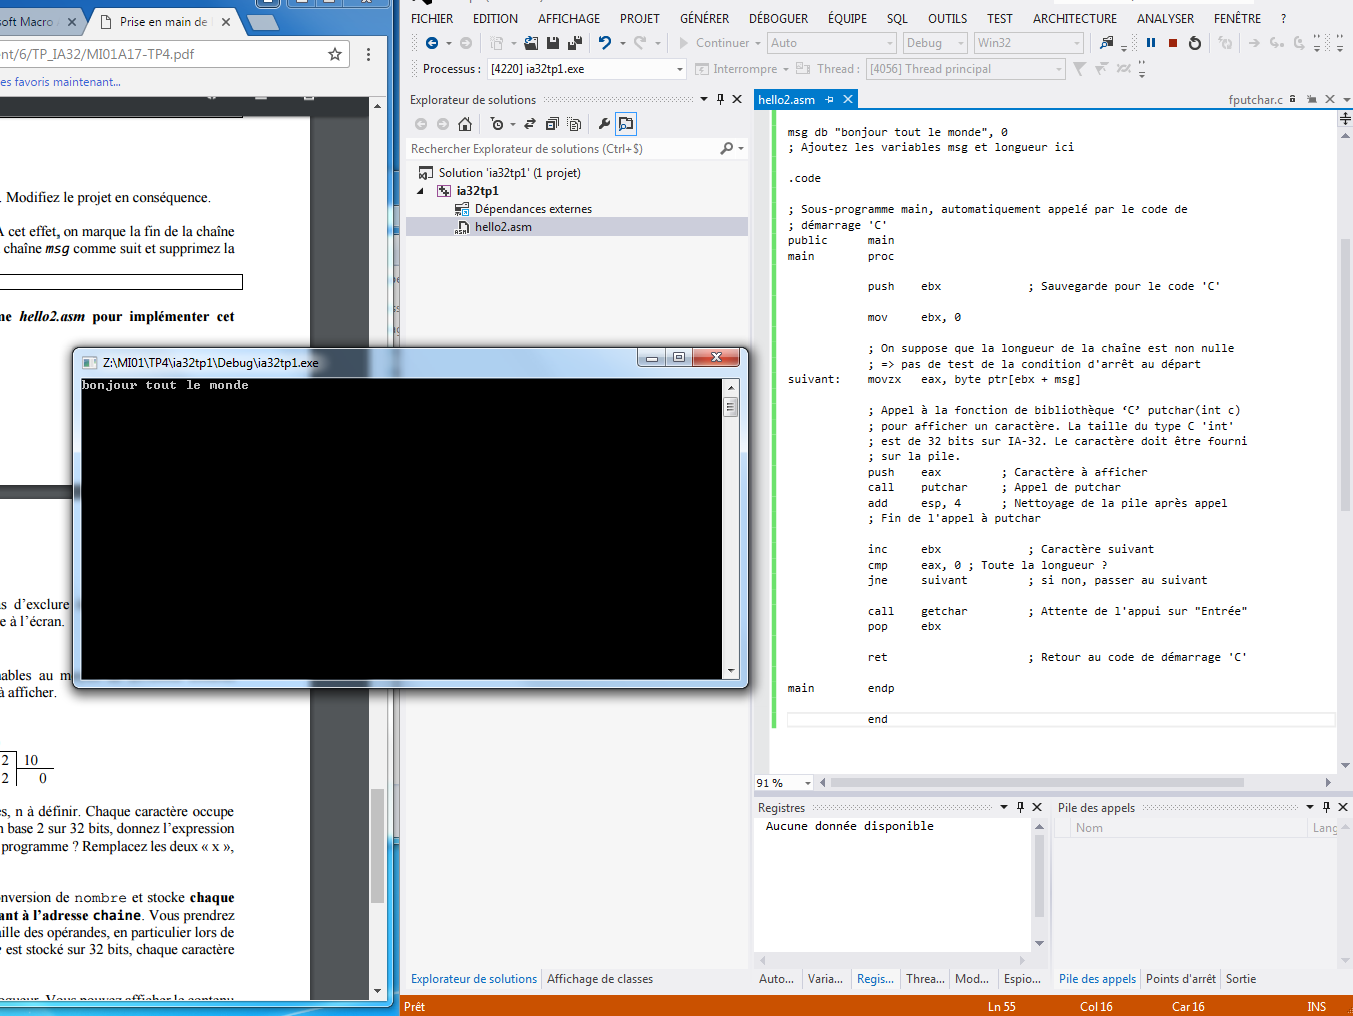
\includegraphics[width=11cm]{Capture4.PNG}
\caption{Programme "hello2"}
\end{figure}

\section{Exercice : conversion et afficahge de nombres}

\subsection{Conversion d'un nombre non signé en base 10}


Dans ce programme on cherche à convertir et afficher des nombres en différentes bases.
Pour cela on utiliser une chaine de caractère de taille n pour stocker la conversion de nombre.
Sachant nombre exprimé en base 2 sur 32 bits. Sa valeur maximale serat donc FFFFFFFFh soit $2^{32}$.
\\ Nous souhaitons convertir le tout en base 10, on résout donc $2^{32}=10^n$.
\\ $2^{32}=10^n$
\\ $32*ln(2) = n*ln(10)$
\\ $n=\frac{32*ln(2)}{ln(10)}$
\\
\\ $n=9.63295986125$
\\
\\ ${\lceil}n{\rceil}=10$
\\
\\ On aura donc besoin d'au plus 10 caractères pour afficher un nombre de 32bits en décimal.

Pour convertir on utilisera la méthode des divisions successive qui fonctionne pour les entiers non signés.
On divise donc successivement l'entier par la base de conversion,
on stocke les restes et on divise le résultat jusqu'à ce que le resultat de la division soit égale a 0.

\begin{lstlisting}
title conversion.asm

.686
.model 		flat, c

extern      putchar:near
extern      getchar:near

.data

nombre      dd      95c8ah          ; Nombre a convertir
chaine      db      10 dup(?)       ; longueur maximale n de la chaine

.code

; Sous-programme main, automatiquement appele par le code de
; demarrage 'C'
public      main
main        proc
			push 	eax							; sauvegarde des registres
			push  ebx             ; Sauvegarde pour le code 'C'

			xor		ebx, ebx
			xor		eax, eax
			mov		ecx, 10         ;base dans laquelle on souhaite convertir la variable nombre
			mov		eax, [nombre]

suivant :		xor 	edx, edx
			div	ecx                ; on divise eax (nombre) par ecx (ici 10)
			mov		[chaine+ebx], dl ; le reste est placé dans le registre edx (le reste sera toujours inferieur a 32 donc il occupera donc toujours au plus les 4 premiers bits de dl) chaque case de chaine étant de 1 octet on copie le registre dl (de 1 octet aussi) dans notre case mémoire de chaine
      inc		ebx              ; on incrémente ebx pour qu'a la prochaine occurence, dl soit placé dans la case mémoire suivante
			cmp		eax, 0           ; si le resultat de la division (registre eax) est 0 alors la conversion est terminé sinon on continue
			jne		suivant

			call    getchar         ; Attente de l'appui sur "Entree"
			pop     ebx
      ret                     ; Retour au code de demarrage 'C'

main       endp

end


\end{lstlisting}

La chaine contient les chiffres brut. Mais putchar affiche les caractères avec la table ASCII.
\\Le caractere 0 ne correspond pas au chiffre 0 dans la table ASCII. On ajoute donc "O" (soit le numero du caractere "0" dans la table ASCII) a nos chiffres pour les faire correspondre aux bon caractere et donc les afficher correctement.

\subsection{Affichage du nombre}

\begin{lstlisting}
; Sous-programme main, automatiquement appele par le code de
; demarrage 'C'
public      main
main        proc
			push 	eax							; sauvegarde des registres
			push  ebx             ; Sauvegarde pour le code 'C'

			xor		ebx, ebx
			xor		eax, eax
			mov		ecx, 10
			mov		eax, [nombre]

suivant :		xor 	edx, edx
			div	ecx
			mov		[chaine+ebx], dl
      inc		ebx
			cmp		eax, 0
			jne		suivant
			dec		ebx             ; on reprend le programme précédent et on decremente ebx pour avoir le bon nombre de chiffres de notre nombre converti.


affichage : movzx   eax, byte ptr[ebx + chaine] on met dans le registre eax un cara caractere de chaine a chaque iteration. On commence par la fin (ici ebx est égale l'index du dernier caractere de chaine)

			add			eax, "0"        ; on ajoute le numero du caractere '0' a notre chiffre pour l'afficher correctement
      push   	eax         		; on ajoute sur la pile le caractere a afficher
      call    putchar     		; Appel de putchar
      add     esp, 4      		; Nettoyage de la pile apres appel
  		dec     ebx             ; Caractere precedent
	    cmp     ebx, 10 				; on compare ebx a 10. Quand ebx est égale a 0 on est au debut de la chaine on a donc affiche le dernier caractere.
      jb     	affichage       ; si on decremente encore ebx sera égale a FFFFFFFFh. Le nombre maximum que peut contenir ebx est le nombre maximum de caractere (ici 10, si il est superieur a 10 c'est qu'il est égale a FFFFFFFFh)
			call    getchar         ; Attente de l'appui sur "Entree"
			pop     ebx
      ret                     ; Retour au code de demarrage 'C'

main       endp

end


\end{lstlisting}


\subsection{Affichage du signe}

La méthode actuellement implémentée ne fonctionne pas pour les nombres négatifs.
Pour qu'elle fonctionne nous devons d'abord réaliser un test permettant de
déterminer si le nombre est négatif ou non.
Si il l'est,on affiche le caractere "-", on prendre son opposé
et on lance le programme déjà conçu précédement

\begin{lstlisting}
.data

nombre      dd      -95c8ah          ; Nombre a convertir
chaine      db      32 dup(?)       ; Remplacer xx par la longueur maximale n de la chaine

.code

; Sous-programme main, automatiquement appele par le code de
; demarrage 'C'
public      main
main        proc
			push 	eax				      ; sauvegarde des registres
			push  ebx             ; Sauvegarde pour le code 'C'

			xor		ebx, ebx
			xor		eax, eax
			mov		ecx, 35
			mov		eax, [nombre]
			cmp 	eax, 0        ;on compare le nombre a 0
			jge 	suivant       ;si il est positif ou nul on ne fait rien et on passe a la conversetion directement
			dec 	eax           ;si le nombre est negatif on le converti en son oppose en decrementant 1
			not 	eax           ;et avec l'operation not
			push 	eax				    ;sauvegarde des registres eax et ecx avant l'appel de putchar
			push	ecx
			push  "-"           ; on affiche le - car le nombre est negatif
      call    putchar     ; Appel de putchar
      add     esp, 4      ; Nettoyage de la pile apres appel
			pop ecx             ; on recupere les registres eax et ebx sauvegardé dans la pile
			pop eax

suivant :		xor 	edx, edx
			div	ecx
			mov		[chaine+ebx], dl
      inc		ebx
			cmp		eax, 0
			jne		suivant
			dec		ebx


affichage : movzx   eax, byte ptr[ebx + chaine]

			add			eax, "0"
      push   	eax         		; Caractere a afficher
      call    putchar     		; Appel de putchar
      add     esp, 4      		; Nettoyage de la pile apres appel
  		dec     ebx             ; Caractere suivant
	    cmp     ebx, 10 				; Toute la longueur ?
      jb     	affichage       ; si non, passer au suivant
			call    getchar         ; Attente de l'appui sur "Entree"
			pop     ebx
      ret                     ; Retour au code de demarrage 'C'

main       endp

end
\end{lstlisting}
\subsection{Base quelconque entre 2 et 36}


On veut donc pouvoir convertir un nombre dans n'importe quelle base entre 2 et 36,
pour cela il suffit de réaliser la division par cette base.
De plus on n'utilisera pas la table ASCI mais une chaîne de caractères composée des caractères allant de 0 à 9 puis de A à Z.
Cette chaîne contient donc tous les digit possibles pour écrire des nombes allant de la base 2 à la base 36.
Pour déterminer quel caractère il faut afficher on utilisera un pointeur
sur cette chaine de caractère qui se déplacera en fonction du résultat de la division.


On aura besoin au maximum d'afficher 32 caractères, la chaîne doit donc avoir pour longueur 32 octets.


\begin{lstlisting}
; conversion.asm
;
; MI01 - TP Assembleur 1
;
; Affiche un nombre de 32 bits sous forme lisible

title conversion.asm

.686
.model 		flat, c

extern      putchar:near
extern      getchar:near

.data

nombre      dd      95c8ah          ; Nombre a convertir
chaine      db      32 dup(?)       ; Remplacer xx par la longueur maximale n de la chaine
chiffres 		db 			"0123456789ABCDEFGHIJKLMNOPQRSTUVWXYZ"

.code

; Sous-programme main, automatiquement appele par le code de
; demarrage 'C'
public      main
main        proc
			push 	eax				; sauvegarde des registres
			push  ebx             ; Sauvegarde pour le code 'C'

			xor		ebx, ebx
			xor		eax, eax
			mov		ecx, 35
			mov		eax, [nombre]
			cmp 	eax, 0
			jge 	suivant
			dec 	eax
			not 	eax
			push 	eax				    ; sauvegarde des registres
			push	ecx
			push  "-"           ; on affiche le - si le nombre est negatif
      call    putchar     ; Appel de putchar
      add     esp, 4      ; Nettoyage de la pile apres appel
			pop ecx
			pop eax

suivant :		xor 	edx, edx
			div	ecx
			mov		[chaine+ebx], dl
      inc		ebx
			cmp		eax, 0
			jne		suivant
			dec		ebx


affichage : movzx   eax, byte ptr[ebx + chaine]

			lea			edx, [chiffres + eax]
      push   	[edx]         	; Caractere a afficher
      call    putchar     		; Appel de putchar
      add     esp, 4      		; Nettoyage de la pile apres appel
  		dec     ebx             ; Caractere suivant
	    cmp     ebx,32 					; Toute la longueur ?
      jb     	affichage       ; si non, passer au suivant
			call    getchar         ; Attente de l'appui sur "Entree"
			pop     ebx
      ret                     ; Retour au code de demarrage 'C'

main       endp

end

\end{lstlisting}


\medskip

En base 35,  95c8ah est égale à EASY

\end{document}
